\section{unode Strukturreferenz}
\label{structunode}\index{unode@{unode}}
{\tt \#include $<$hashtab.h$>$}

Zusammengeh\"{o}rigkeiten von unode:\begin{figure}[H]
\begin{center}
\leavevmode
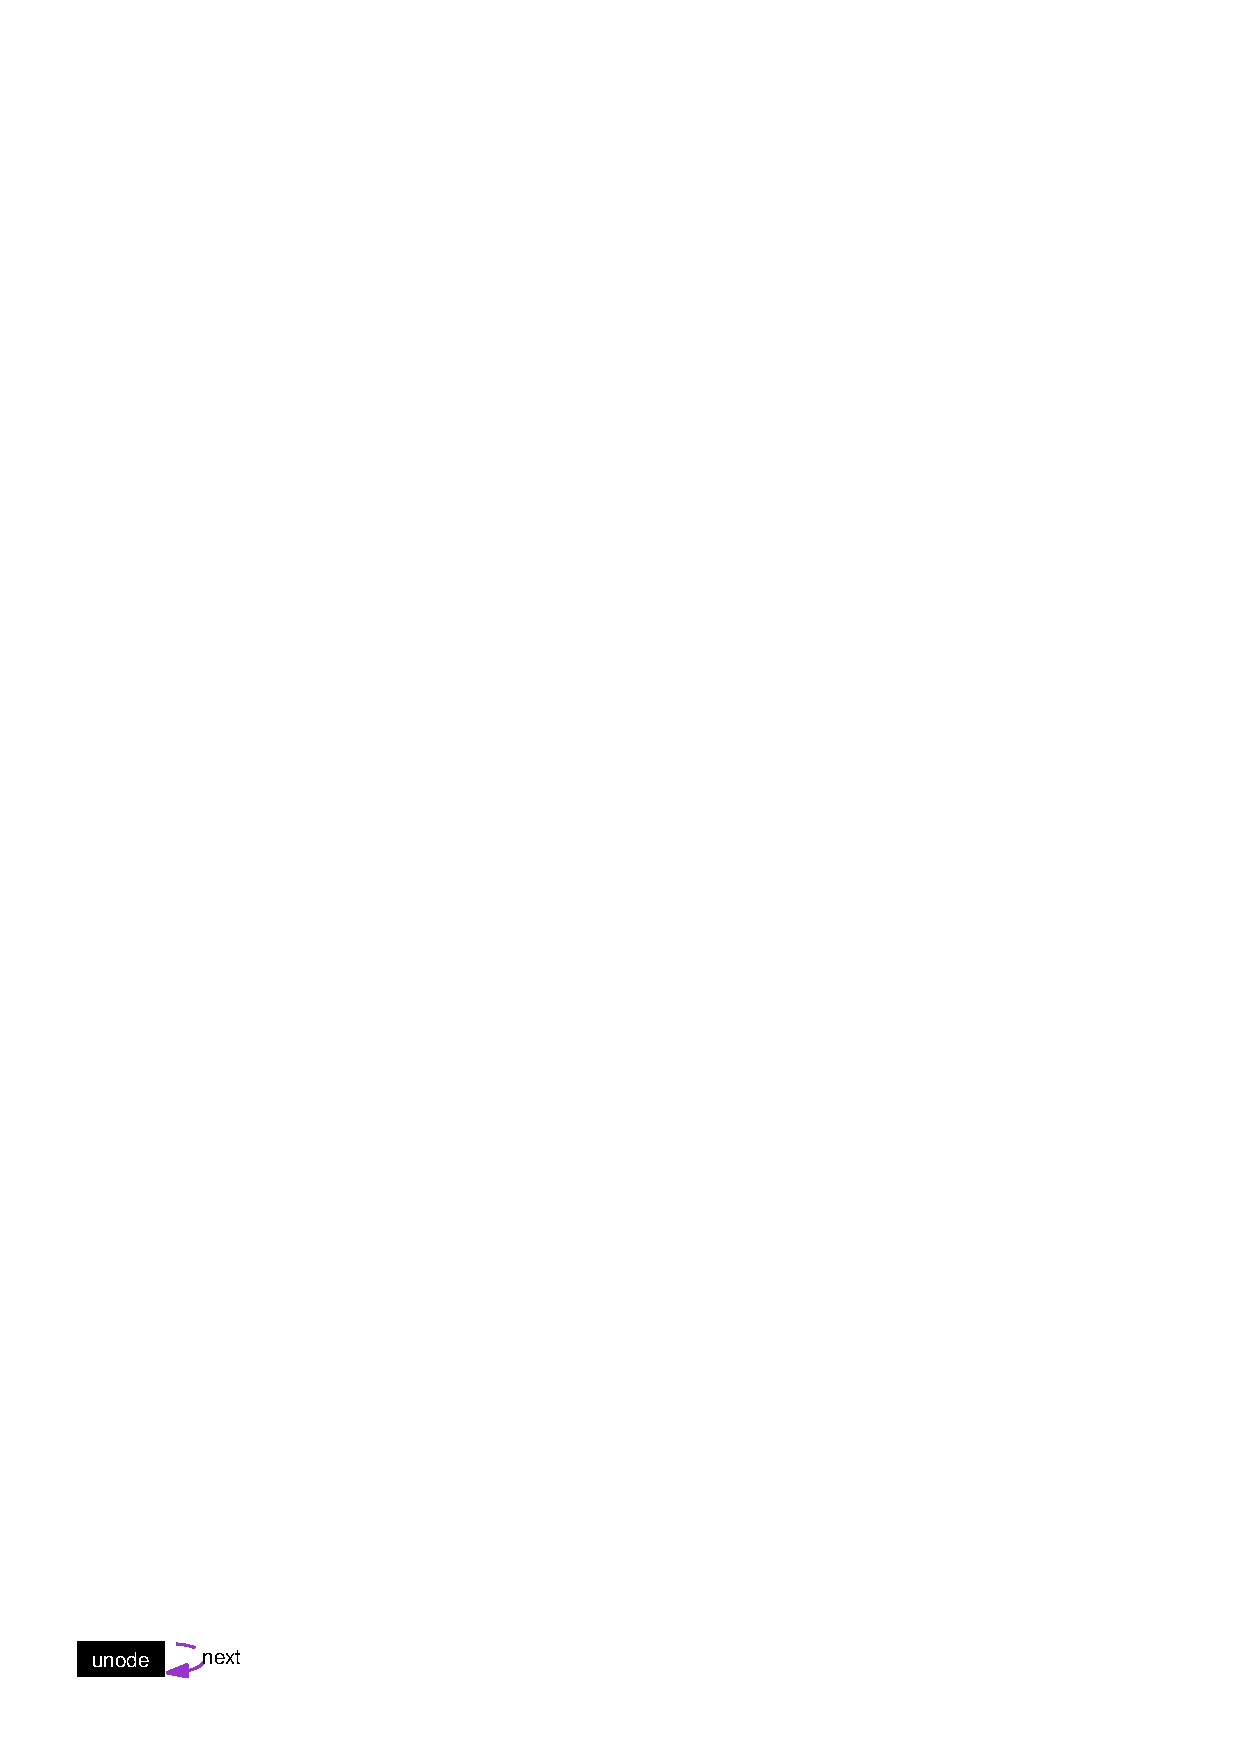
\includegraphics[width=59pt]{structunode__coll__graph}
\end{center}
\end{figure}
\subsection*{Datenfelder}
\begin{CompactItemize}
\item 
char $\ast$ {\bf string}
\item 
int {\bf flag}
\item 
u\_\-long {\bf count}
\item 
u\_\-long {\bf files}
\item 
u\_\-long {\bf entry}
\item 
u\_\-long {\bf exit}
\item 
double {\bf xfer}
\item 
{\bf unode} $\ast$ {\bf next}
\end{CompactItemize}


\subsection{Ausf\"{u}hrliche Beschreibung}




Definiert in Zeile 36 der Datei hashtab.h.

\subsection{Dokumentation der Datenelemente}
\index{unode@{unode}!count@{count}}
\index{count@{count}!unode@{unode}}
\subsubsection{\setlength{\rightskip}{0pt plus 5cm}u\_\-long {\bf unode::count}}\label{structunode_3c9d9be50f4911615af8e7de965a7435}




Definiert in Zeile 38 der Datei hashtab.h.

Wird benutzt von all\_\-urls\_\-page(), dump\_\-all\_\-urls(), new\_\-unode(), put\_\-unode(), top\_\-entry\_\-table() und top\_\-urls\_\-table().\index{unode@{unode}!entry@{entry}}
\index{entry@{entry}!unode@{unode}}
\subsubsection{\setlength{\rightskip}{0pt plus 5cm}u\_\-long {\bf unode::entry}}\label{structunode_8799c3c150906874e134a2cc3ccce10d}




Definiert in Zeile 40 der Datei hashtab.h.

Wird benutzt von put\_\-unode(), top\_\-entry\_\-table() und update\_\-entry().\index{unode@{unode}!exit@{exit}}
\index{exit@{exit}!unode@{unode}}
\subsubsection{\setlength{\rightskip}{0pt plus 5cm}u\_\-long {\bf unode::exit}}\label{structunode_60177f74305a04d4aac550c6b24f8549}




Definiert in Zeile 41 der Datei hashtab.h.

Wird benutzt von put\_\-unode(), top\_\-entry\_\-table() und update\_\-exit().\index{unode@{unode}!files@{files}}
\index{files@{files}!unode@{unode}}
\subsubsection{\setlength{\rightskip}{0pt plus 5cm}u\_\-long {\bf unode::files}}\label{structunode_e804f1505713967ff89aae41783c6be1}




Definiert in Zeile 39 der Datei hashtab.h.\index{unode@{unode}!flag@{flag}}
\index{flag@{flag}!unode@{unode}}
\subsubsection{\setlength{\rightskip}{0pt plus 5cm}int {\bf unode::flag}}\label{structunode_172c31b32a93663cdde52fba42c0343d}




Definiert in Zeile 37 der Datei hashtab.h.

Wird benutzt von all\_\-urls\_\-page(), dump\_\-all\_\-urls(), new\_\-unode(), put\_\-unode(), top\_\-entry\_\-table(), top\_\-urls\_\-table(), update\_\-entry() und update\_\-exit().\index{unode@{unode}!next@{next}}
\index{next@{next}!unode@{unode}}
\subsubsection{\setlength{\rightskip}{0pt plus 5cm}struct {\bf unode}$\ast$ {\bf unode::next}}\label{structunode_84a3ee805e5f7a6011c4c9c5866a27b6}




Definiert in Zeile 43 der Datei hashtab.h.

Wird benutzt von del\_\-ulist(), find\_\-url(), load\_\-url\_\-array(), put\_\-unode(), update\_\-entry() und update\_\-exit().\index{unode@{unode}!string@{string}}
\index{string@{string}!unode@{unode}}
\subsubsection{\setlength{\rightskip}{0pt plus 5cm}char$\ast$ {\bf unode::string}}\label{structunode_7e4e6f981e97f717739e1844247456a0}




Definiert in Zeile 36 der Datei hashtab.h.

Wird benutzt von all\_\-urls\_\-page(), del\_\-ulist(), dump\_\-all\_\-urls(), find\_\-url(), new\_\-unode(), put\_\-unode(), top\_\-entry\_\-table(), top\_\-urls\_\-table(), update\_\-entry() und update\_\-exit().\index{unode@{unode}!xfer@{xfer}}
\index{xfer@{xfer}!unode@{unode}}
\subsubsection{\setlength{\rightskip}{0pt plus 5cm}double {\bf unode::xfer}}\label{structunode_b0e69efc030906335d50a264aa2d2878}




Definiert in Zeile 42 der Datei hashtab.h.

Wird benutzt von all\_\-urls\_\-page(), dump\_\-all\_\-urls(), put\_\-unode() und top\_\-urls\_\-table().

Die Dokumentation f\"{u}r diese Struktur wurde erzeugt aufgrund der Datei:\begin{CompactItemize}
\item 
oosalizer/{\bf hashtab.h}\end{CompactItemize}
